
\documentclass[a4paper,11pt]{article}

\usepackage{amsmath}
\usepackage{graphicx}
\usepackage{url}

% Hyperlink contents page
\usepackage{hyperref}
\hypersetup{
	colorlinks,
	citecolor=black,
	filecolor=black,
	linkcolor=black,
	urlcolor=black
}

% Tables
\usepackage{tabularx}
\usepackage{multirow}
\newcolumntype{Y}{>{\centering\arraybackslash}X}

% No indent on new paragraphs
\setlength{\parindent}{0mm}
\setlength{\parskip}{0.2cm}

% Tables
\usepackage{array}
\newcolumntype{L}[1]{>{\raggedright\let\newline\\\arraybackslash\hspace{0pt}}m{#1}}
\newcolumntype{C}[1]{>{\centering\let\newline\\\arraybackslash\hspace{0pt}}m{#1}}
\newcolumntype{R}[1]{>{\raggedleft\let\newline\\\arraybackslash\hspace{0pt}}m{#1}}


\begin{document}

\title{Spaghetti Bridge Investigation}
\author{Ben Anderson}
\date{\today}
\maketitle

\pagebreak

\tableofcontents
\pagebreak


\section{Abstract}

An investigation into bridge design, accompanied by the construction and testing
of a bridge produced from spaghetti, with the aim of achieving the highest load
to mass ratio in the class.




\section{Research}

\subsection{Forces}

\begin{figure}
\begin{center}
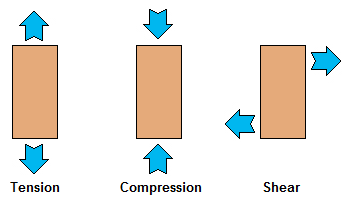
\includegraphics[width=8cm]{figures/forces.png}
\end{center}
\caption{Tension, compression, and shear forces}
\label{research:forces}
\end{figure}

The most important consideration in designing a bridge is to enable it to
carry a sufficient load in order to prevent it from collapsing.
Bridges are designed in order to reduce the forces acting in different
components when a load force is applied, because applying stresses on a
component beyond what is it capable of withstanding will likely cause the bridge
to fail.

There are two main forces which components in a bridge will experience: tension
and compression. See Figure \ref{research:forces}.


\subsubsection{Tension}

When a component of a bridge is under tension, the component experiences a
pulling force exerted in opposite directions on each end.

Tension is sustained by electrostatic attraction between atoms in the material.
If the tension force experienced by the component exceeds the maximum restoring
force that can be provided by this electrostatic attraction, the component will
fail.


\subsubsection{Compression}

Compression is where a component of the bridge experiences a ``pushing" force
inwards.

Compression is sustained by electrostatic repulsion between atoms in the
material.
It may cause the material to buckle and fail if the compression force exceeds
the maximum the material can withstand.


\subsubsection{Shear}

A shear force is one with a component in the plane perpendicular to the
material's surface.


\subsubsection{Torsion}

A torsion force is one that exerts a twisting moment in a component of the
bridge.


\subsubsection{Young's Modulus}

Young's modulus is a measure of a material's ability to withstand tension forces
(a measure of tensile strength), and is defined as the ratio of stress over
strain in a plane parallel to the material.

Spaghetti has relatively high Young's Modulus, with a value of 69 GPa,
comparable to that of aluminium.


\subsubsection{Compressive Strength}

The compressive strength of spaghetti, although still relatively high, is
smaller than its tensile strength.
Spaghetti can withstand approximately 7.5 times less force under compression
when compared to tension.

Spaghetti's compressive strength also depends upon the length of the segment, as
shorter pieces are able to withstand higher compression forces before buckling
and breaking.
This can be demonstrated by observing the formula for buckling strength:

$$
F = k \frac{d^4}{l^2}
$$

Where $d$ is the diameter of the spaghetti strand, $l$ its length, and $k$ the
constant of proportionality.

$F$ is inversely proportional to the square of the length of the spaghetti
strand.
Thus halving the length of a piece of spaghetti quadruples its buckling
strength.


\subsubsection{Shear Strength}

Shear strength is a measure of a material's ability to withstand shear forces (a
measure of shear strength), and is defined as the ratio of shear stress over
shear strain in a plane perpendicular to the material.

Spaghetti has a relatively low shear strength, with a value of only 0.4 GPa,
compared to aluminium's 25.5 GPa.
This is about 99.42\% less than its tensile strength.


\subsubsection{Torsion Strength}

Spaghetti also has a relatively low torsion strength, shattering if exposed to
such forces.


\subsubsection{Conclusions}

From this information regarding the tensile and shear strength of spaghetti, we
can conclude that a bridge design that maximises tension and compression forces
on the spaghetti, and minimises shearing an torsion forces, will be most
effective in achieving a high load to mass ratio.

Additionally, the compressive strength of spaghetti is approximately 7.5 times
worse than its tensile strength. Thus maximising tension forces over compression
will also aid in increasing the bridge's load to mass ratio.


\subsection{Features of Bridges}

There are many varied bridge designs that exist, but most have some common
features due to their proven strength.


\subsubsection{Triangles}

Most bridges feature triangular shapes throughout the design, due to the
inherent structural characteristics unique to this polygon.

Triangles are inherently strong because they are the only polygon in which the
a change in any of the 3 angles must cause a change in its corresponding side.
Thus the force required to change a triangle's shape is equivalent to the force
required to deform a side of the triangle.
The strength of other polygons depends only the strength of their corners (for
example, a rectangle can become a parallelogram through only a change in the
corner angles).

This inherent strength in their geometry has resulted in their pervasive use
throughout bridge design.


\subsubsection{Arches}

\begin{figure}
\begin{center}
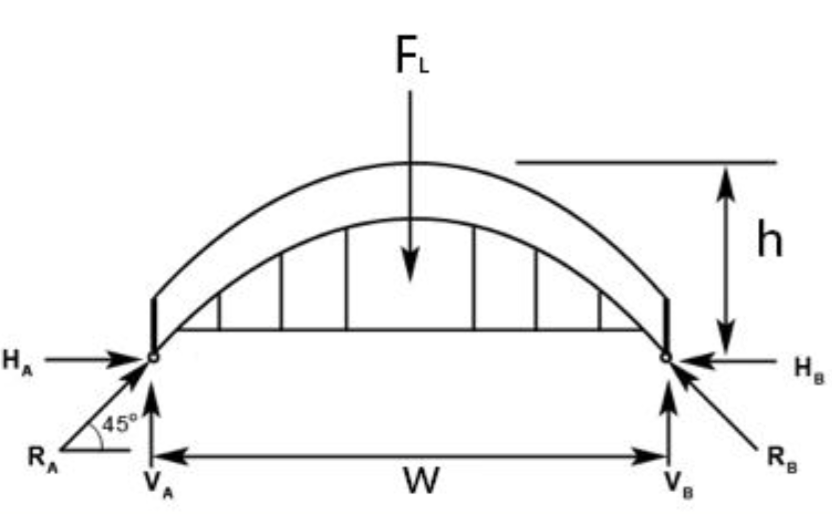
\includegraphics[width=8cm]{figures/arch.png}
\end{center}
\caption{Forces acting on an arch}
\label{research:arch}
\end{figure}

Many bridge designs also depend on the strength of semi-cirular or parabolic
arcs in distributing compressive forces to abutments on the ground either side
of the bridge.

A load force placed on an arch induces a compression force within each segment
of the arch, eventually exerting a force on the abutments, which in turn exert
a reaction force on the bridge.
This distributes the load force to the ground.

See Figure \ref{research:arch} for a diagramatic representation of these forces.
The load force $F_L$ causes compression in the arch, causing the abutments to
exert reaction forces $R_A$ and $R_B$ on the bridge.


\subsection{Bridge Designs}

Of the innumerous bridge designs in existence, only a few were decidedly
feasible to construct from spaghetti.


\subsection{Beam Bridge}

A beam bridge is one of the simplest designs in existence.


\subsection{Truss Bridge}

\subsubsection{Pratt Truss}

\subsubsection{Warren Truss}

\subsection{Arch Bridge}

These forces cause the arch to push outwards horizontally on its base, called
thrust.
As the height of the arch ($h$ in the diagram) decreases, the thrust increases.
Thrust must be kept at a managable level in order to prevent the bridge from
collapsing.
This is usually achieved either through external bracing (abutments), or
internal spokes.




\section{Testing Tensile Strength}

The first stage of pre-testing was to decide on which brand and style of
spaghetti to use in constructing the bridge.
This decision was based on two tests.

This first test measures the maximum tension force a bundle of spaghetti can
withstand before breaking.


\subsection{Equipment}

\begin{itemize}
\item GLX electronic force metre and associated power pack
\item Varying spaghetti brands and styles (listed under the results section)
\item 2 tables of the same height
\item 2 heat proof mats
\item Electronic scales
\end{itemize}


\subsection{Procedure}

\begin{enumerate}
\item Place two desks of the same height next to each other, separated by a 15
	cm gap.
\item Place a heat proof mat at the edge of each desk to ensure corners of the
	desk are square, rather than rounded. This ensures there is a single
	point around which the spaghetti pivots when it bends.
\item Turn on the GLX force metre and calibrate it.
\item \label{tensile:start} Select one brand and style of spaghetti to test.
\item \label{tensile:inner-start} Gather 5 pieces of this particular spaghetti
	and cut each piece to 25 cm.
\item Record the mass of the bundle.
\item Form a circular bundle of 5 pieces of spaghetti and place it over the gap,
	centering it such that 5 cm of spaghetti overlaps the desks on each side.
\item Place the spaghetti through the hook on the force metre.
\item Gradually pull down vertically on the force metre, stopping once the
	spaghetti breaks.
\item \label{tensile:inner-end} Record the maximum force the spaghetti could
	withstand before breaking.
\item \label{tensile:end} Repeat steps \ref{tensile:inner-start} to
	\ref{tensile:inner-end} an additional 2 times for a total of 3 trials.
\item Repeat steps \ref{tensile:start} to \ref{tensile:end} with another
	style or brand of spaghetti, stopping once all available types have been
	exhausted.
\end{enumerate}


\subsection{Diagram}

A diagram of the testing setup is below:

\vspace{5cm}


\subsection{Results}

Zafarelli Regular Spaghetti:

\begin{center}
\begin{tabular}{|c|c|c|}
\hline
Trial & Mass ($\times 10^{-3}\mbox{ kg}$) & Force (N) \\
\hline
1       & 5.10 & 2.9 \\
2       & 5.11 & 2.7 \\
3       & 5.10 & 2.8 \\
\hline
Average & 5.10 & 2.80 \\
\hline
\end{tabular}
\end{center}

Barilla Regular Spaghetti:

\begin{center}
\begin{tabular}{|c|c|c|}
\hline
Trial & Mass ($\times 10^{-3}\mbox{ kg}$) & Force (N) \\
\hline
1       & 5.08 & 2.9 \\
2       & 5.04 & 2.8 \\
3       & 5.06 & 2.8 \\
\hline
Average & 5.06 & 2.83 \\
\hline
\end{tabular}
\end{center}

Coles Regular Spaghetti:

\begin{center}
\begin{tabular}{|c|c|c|}
\hline
Trial & Mass ($\times 10^{-3}\mbox{ kg}$) & Force (N) \\
\hline
1       & 5.01 & 3.0 \\
2       & 5.05 & 2.7 \\
3       & 5.07 & 3.0 \\
\hline
Average & 5.04 & 2.90 \\
\hline
\end{tabular}
\end{center}

San Remo Wholemeal Spaghetti:

\begin{center}
\begin{tabular}{|c|c|c|}
\hline
Trial & Mass ($\times 10^{-3}\mbox{ kg}$) & Force (N) \\
\hline
1       & 5.51 & 2.6 \\
2       & 5.48 & 2.5 \\
3       & 5.46 & 2.5 \\
\hline
Average & 5.48 & 2.53 \\
\hline
\end{tabular}
\end{center}

Coles Thin Spaghetti:

\begin{center}
\begin{tabular}{|c|c|c|}
\hline
Trial & Mass ($\times 10^{-3}\mbox{ kg}$) & Force (N) \\
\hline
1       & 3.42 & 1.6 \\
2       & 3.58 & 1.7 \\
3       & 3.54 & 1.6 \\
\hline
Average & 3.51 & 1.63 \\
\hline
\end{tabular}
\end{center}

San Remo Thick Spaghetti:

\begin{center}
\begin{tabular}{|c|c|c|}
\hline
Trial & Mass ($\times 10^{-3}\mbox{ kg}$) & Force (N) \\
\hline
1       & 5.58 & 4.1 \\
2       & 5.53 & 4.5 \\
3       & 5.62 & 3.6 \\
\hline
Average & 5.58 & 4.07 \\
\hline
\end{tabular}
\end{center}

San Remo Tubular Spaghetti:

\begin{center}
\begin{tabular}{|c|c|c|}
\hline
Trial & Mass ($\times 10^{-3}\mbox{ kg}$) & Force (N) \\
\hline
1       & 8.06 & 7.2 \\
2       & 7.95 & 7.3 \\
3       & 7.60 & 7.9 \\
\hline
Average & 7.87 & 7.47 \\
\hline
\end{tabular}
\end{center}


\subsection{Load to Mass}

For each type of spaghetti, the load to mass ratio was calculated. These results
are shown in the table below:

\begin{center}
\makebox[\textwidth][c]{
\begin{tabular}{|C{0.25\textwidth}|C{0.2\textwidth}|C{0.2\textwidth}|C{0.2\textwidth}|C{0.15\textwidth}|}
\hline
Spaghetti & Average Mass ($\times 10^{-3}\mbox{ kg}$) & Average Force (N) &
Effective Load (kg) & Load to Mass \\
\hline
Wholemeal         & 5.48 & 2.53 & 0.25816 & 47.12 \\
Thin              & 3.51 & 1.63 & 0.16633 & 47.39 \\
Zafarelli Regular & 5.10 & 2.80 & 0.28571 & 56.02 \\
Barilla Regular   & 5.06 & 2.83 & 0.28878 & 57.07 \\
Coles Regular     & 5.04 & 2.90 & 0.29592 & 58.71 \\
Thick             & 5.58 & 4.07 & 0.41531 & 74.43 \\
Tubular           & 7.87 & 7.47 & 0.76224 & 96.85 \\
\hline
\end{tabular}
}
\end{center}


\subsubsection{Sample Calculation}

A sample calculation for the load to mass ratio of San Remo tubular spaghetti
is shown below.

Effective load:

$$
\begin{aligned}
F & = ma \\
7.47 & = m \times 9.8 \\
m & = 0.28571\mbox{ kg} \\
\end{aligned}
$$

Load to mass ratio:

$$
\begin{aligned}
& = \frac{0.76224}{7.87 \times 10^{-3}} \\
& = 96.85 \\
\end{aligned}
$$


\subsection{Evaluation}

The data above indicates that, despite San Remo tubular spaghetti being the
heaviest type of spaghetti tested, it had the best load to mass ratio when
subject to a tension force.
This suggests that it would be the most effective form of spaghetti to use in
the construction of our bridge.

In addition, its load to mass ratio was much higher than any other form of
spaghetti tested, indicating that there was likely little to be gained from
using multiple types of spaghetti in the one bridge due to its clear
superiority.




\section{Testing Compressive Strength}

The second test conducted in order to determine which type and brand of
spaghetti to use in constructing our bridge was one that measured the ability
of spaghetti to withstand a compressive force.


\subsection{Equipment}

\begin{itemize}
\item Electronic scales
\item Varying spaghetti brands and styles (listed under the results section)
\end{itemize}


\subsection{Procedure}

\begin{enumerate}
\item Set up the electronic scales and tear it.
\item \label{compression:start} Select a type of spaghetti to test.
\item \label{compression:inner-start} Gather 1 strand of the selected spaghetti.
\item Place one end on the electronic scales and stand it upright, holding the
	other end in your palm.
\item Press down vertically with your hand.
\item \label{compression:inner-end} Record the maximum mass reading on the
	electronic scales before the spaghetti breaks.
\item \label{compression:end} Repeat steps \ref{compression:inner-start} to
	\ref{compression:inner-end} an additional 3 times for a total of 4 trials.
\item Repeat steps \ref{compression:start} to \ref{compression:end} for each
	brand and style of spaghetti.
\end{enumerate}


\subsection{Diagram}

A diagram of the testing setup is below:

\vspace{5cm}


\subsection{Results}

\begin{center}
\makebox[\textwidth][c]{
\begin{tabular}{|c|c|c|c|c|c|}
\hline
\multirow{2}{*}{Spaghetti} & \multicolumn{5}{c|}{Maximum Mass Reading
($\times 10^{-3}\mbox{ kg}$)} \\
\cline{2-6}
& Trial 1 & Trial 2 & Trial 3 & Trial 4 & Average \\
\hline
Wholemeal         & 49  & 52  & 58  & 43  & 50.5  \\
Thin              & 30  & 24  & 39  & 36  & 32.3  \\
Zafarelli Regular & 42  & 60  & 48  & 55  & 51.3  \\
Barilla Regular   & 52  & 45  & 65  & 49  & 52.8  \\
Coles Regular     & 50  & 57  & 62  & 49  & 54.5  \\
Thick             & 63  & 69  & 52  & 71  & 63.8  \\
Tubular           & 128 & 118 & 147 & 130 & 130.8 \\
\hline
\end{tabular}
}
\end{center}


\subsection{Load to Mass}

For each type of spaghetti, the load to mass ratio was calculated. These results
are shown in the table below:

\begin{center}
\makebox[\textwidth][c]{
\begin{tabular}{|C{0.25\textwidth}|C{0.25\textwidth}|C{0.3\textwidth}|C{0.2\textwidth}|}
\hline
Spaghetti & Mass ($\times 10^{-3}\mbox{ kg}$) & Average Compression
($\times 10^{-3}\mbox{ kg}$) & Load to Mass \\
\hline
Wholemeal         & 1.10 & 50.5  & 45.91 \\
Thin              & 0.70 & 32.3  & 46.07 \\
Zafarelli Regular & 1.02 & 51.3  & 50.25 \\
Barilla Regular   & 1.01 & 52.8  & 52.23 \\
Coles Regular     & 1.01 & 54.5  & 53.96 \\
Thick             & 1.12 & 63.8  & 56.92 \\
Tubular           & 1.57 & 130.8 & 83.28 \\
\hline
\end{tabular}
}
\end{center}


\subsubsection{Sample Calculation}

A sample calculation for the load to mass ratio of San Remo tubular spaghetti is
shown below:

$$
\begin{aligned}
& = \frac{130.8 \times 10^{-3}}{1.57 \times{10^{-3}}} \\
& = 83.28 \\
\end{aligned}
$$


\subsection{Evaluation}

The data above indicates that San Remo tubular spaghetti is has the best load
to mass ratio when subject to a compressive force.
Again, this suggests the most effective form of spaghetti to use in the
construction of our bridge is tubular spaghetti.

Tubular spaghetti's load to mass ratio is also significantly superior to any
other type of spaghetti.
Again, this likely suggests that little is to be gained by using multiple types
of spaghetti in the one bridge.




\section{Testing Glues}

The next stage of pre-testing was to decide on which brand and style of glue to
use in constructing the bridge.
This was decided through a test of glue strength under tensile stress.


\subsection{Equipment}

\begin{itemize}
\item GLX force metre and associated power pack
\item Varying brands and styles of glue (listed under the results section)
\item San Remo tubular spaghetti
\item Lengths of string
\item Hot glue gun and associated sticks of glue
\item Table
\end{itemize}


\subsection{Procedure}

\begin{enumerate}
\item For each type of glue to test, glue two strands of tubular spaghetti
	together, end to end, without any overlap. Ensure that a consistent volume
	of glue is used in gluing each of the pairs of spaghetti.
\item Leave all glues to dry for 24 hours.
\item Using the hot glue gun and an excessive volume of glue, attach a length of
	string to each end of each spaghetti pair.
\item Tie a loop knot in one of the string lengths attached to each of the glued
	spaghetti pairs.
\item Set up and calibrate the GLX force metre.
\item \label{glue:start} Select one of the glued spaghetti pairs, and tie the
	other length of string attached to it to a stationary table leg.
\item Thread the hook on the force metre through the loop knot in the other
	length of string.
\item Gradually pull on the force metre horizontally, until the glued join
	between the two pieces of spaghetti fails.
\item \label{glue:end} Record the maximum force required to separate the two
	pieces of spaghetti.
\item Repeat steps \ref{glue:start} to \ref{glue:end} for each glued pair of
	spaghetti strands.
\end{enumerate}


\subsection{Diagram}

A diagram of the testing setup is below:

\vspace{5cm}


\subsection{Results}

\begin{center}
\begin{tabular}{|c|c|}
\hline
Glue & Force (N) \\
\hline
Glue Stick                 & 0.5  \\
UHU Universal Glue         & 5.1  \\
Tarzan Grip 5 Minute Epoxy & 5.6  \\
Bostik Superglue           & 5.9  \\
Selley's Liquid Nails      & 13.8 \\
Araldite 5 Minute Epoxy    & 14.0 \\
Hot Glue                   & 14.1 \\
\hline
\end{tabular}
\end{center}


\subsection{Evaluation}

The above data suggests that hot glue is capable of withstanding the largest
tensile force before breaking.
The second strongest glue is Araldite 5 minute expoxy, only slightly weaker
than hot glue.

In a spaghetti bridge, the main determining factors of its load to mass ratio
are the strength of the design and strength of the spaghetti used to construct
the bridge.
Since the strength of glue used to hold the bridge together is not one of the
most significant factors, our decision on which glue to use can be influenced
by convenience and aesthetic factors.


\subsubsection{Hot Glue}

Hot glue is the most convenient type of glue to use, as it sets almost
immediately.
This enables rapid construction of more difficult designs, as we are able to
simply hold pieces of spaghetti in place for a short while as the glue sets.
This is not possible for glues that take longer to set, such as the Bostik
Superglue or Selley's Liquid Nails.

Despite this, hot glue also has appreciable disadvantages when considering
aesthetics.
Without proper care, it can leave traces of glue on segments of spaghetti which
are difficult to remove without risking the destruction of the spaghetti.
It also leaves long, thin strands of residue glue which, if not removed,
detract from the overall aesthetics of the design.

Another significant disadvantage of hot glue is that joints formed using it were
found to be reasonably flexible, bending and twisting when force was applied.
This lack of rigidity at joints in our bridge, if constructed with hot glue,
would likely cause it to bend and sag when placed under high load.
This would unevenly distribute tension and compression forces amongst the
segments of spaghetti in the design, decreasing the ability of the bridge to
support high loads.


\subsubsection{Epoxy}

The Araldite 5 minute epoxy is less convenient than hot glue, as it takes 5
minutes to set and consists of two separate liquid components which must be
mixed and then applied to the structure.

Despite this, its high viscosity (especially when compared to Selley's Liquid
Nails, which was of a comparable strength) made it more convenient than some
alternatives, as it remained in its intended position once applied.

Additionally, joints constructed with epoxy were found to be extremely rigid,
not moving when we applied a variety of bending and twisting forces.
This would allow our bridge to remain rigid, bending and sagging little under
high loads, sustaining an even distribution of tension and compression forces.


\subsubsection{Chosen Combination}

In considering the above factors, we decided to use a combination of hot glue
and epoxy in our bridge.

The most significant factor influencing this decision was the glues' significant
strength when compared to the available alternatives.
Hot glue and epoxy were the two strongest glues tested.

For more simpler joints in our final design, such as joints along the base, it
was decided that a judicious coating of epoxy would suffice in securing the
structure.
Our use of epoxy over hot glue is justified by the fact that both glues
displayed an extremely similar level of strength, yet joints formed using epoxy
were far more rigid than those with hot glue. This rigidity is very beneficial
to the overall design, as discussed above.

More complicated joints, such joining the spokes to the arch and base, would
be completed first by using a small amount of hot glue to hold the segments of
spaghetti in place, and then applying a coat of epoxy to increase the rigidity
of the joint, thus improve the rigidity of the overall structure.




\section{Testing Bundle Sizes}

In the final design of our bridge, we intended to use bundles of spaghetti of
different sizes for different parts of the bridge.
The next stage of pre-testing was to determine which bundle sizes have the
highest load to mass ratio.

This test measured the tensile strength of varying sized bundles of tubular
spaghetti.


\subsection{Equipment}

\begin{itemize}
\item GLX force metre and associated power pack
\item San Remo tubular spaghetti
\item 2 tables
\item 2 heat proof mats
\item String
\item Electronic scales
\end{itemize}


\subsection{Procedure}

\begin{enumerate}
\item Place two desks of the same height next to each other, separated by a 15
	cm gap.
\item Place a heat proof mat on the edge of each desk (due to the same reason as
	in previous tests).
\item Turn on the GLX force metre and calibrate it.
\item \label{bundle:start} Start with a bundle size of 1 spaghetti.
\item Cut each piece of spaghetti in the bundle to 25 cm.
\item Record the mass of the bundle.
\item \label{bundle:inner-start} Place the bundle across the gap, ensuring it
	is centred so that 5 cm of spaghetti overlaps the table on each side.
\item Tie a loop of string around the bundle of spaghetti.
\item Hook the force metre around the loop of string.
\item Gradually pull down vertically on the force metre, stopping once the
	bundle breaks.
\item \label{bundle:inner-end} Record the maximum force the bundle withstood
	before breaking.
\item \label{bundle:end} Repeat steps \ref{bundle:inner-start} to
	\ref{bundle:inner-end} an additional 2 times for a total of 3 trials.
\item Repeat steps \ref{bundle:start} to \ref{bundle:end}, increasing the bundle
	size by 1, stopping when a bundle size of 8 is reached.
\end{enumerate}


\subsection{Results}

The force each bundle size could withstand before breaking:

\begin{center}
\begin{tabular}{|c|c|c|c|c|}
\hline
\multirow{2}{*}{Bundle Size} & \multicolumn{4}{c|}{Force (N)} \\
\cline{2-5}
& Trial 1 & Trial 2 & Trial 3 & Average \\
\hline
1 & 2.41 & 2.40 & 2.40 & 2.40 \\
2 & 4.01 & 4.01 & 3.99 & 4.00 \\
3 & 6.78 & 6.80 & 6.82 & 6.80 \\
4 & 8.50 & 8.51 & 8.50 & 8.50 \\
5 & 10.3 & 10.2 & 10.3 & 10.3 \\
6 & 12.8 & 12.8 & 12.7 & 12.8 \\
7 & 17.5 & 17.3 & 17.4 & 17.4 \\
8 & 18.6 & 18.5 & 18.5 & 18.5 \\
\hline
\end{tabular}
\end{center}

The load to mass ratio of each bundle:

\begin{center}
\makebox[\textwidth][c]{
\begin{tabular}{|C{0.2\textwidth}|C{0.2\textwidth}|C{0.2\textwidth}|C{0.2\textwidth}|C{0.2\textwidth}|}
\hline
Bundle Size & Mass ($\times 10^{-3}\mbox{ kg}$) & Average Force (N) & Effective
Load (kg) & Load to Mass \\
\hline
1 & 1.6  & 2.40 & 0.2449 & 153 \\
2 & 3.3  & 4.00 & 0.4082 & 124 \\
3 & 5.0  & 6.80 & 0.6939 & 139 \\
4 & 6.4  & 8.50 & 0.8673 & 136 \\
5 & 8.1  & 10.3 & 1.051  & 130 \\
6 & 9.8  & 12.8 & 1.306  & 133 \\
7 & 11.6 & 17.4 & 1.776  & 153 \\
8 & 12.9 & 18.5 & 1.888  & 146 \\
\hline
\end{tabular}
}
\end{center}

\begin{figure}
\begin{center}
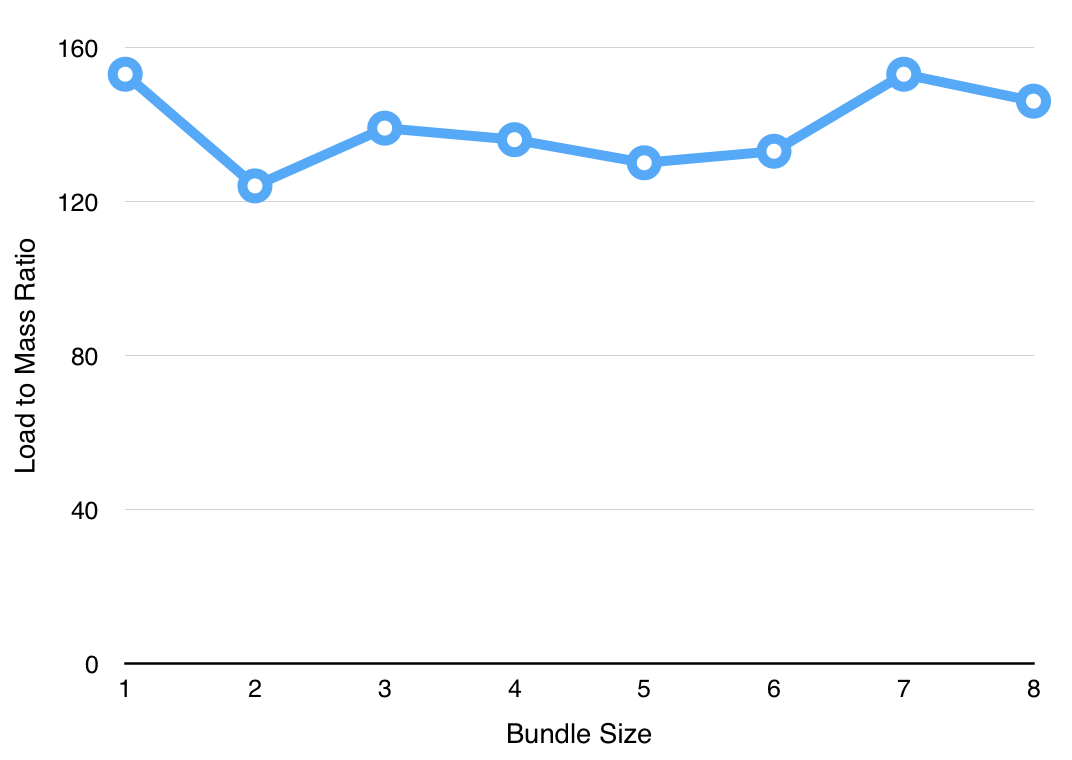
\includegraphics[width=10cm]{figures/bundles.png}
\end{center}
\caption{Load to mass ratio vs. bundle size}
\label{bundles:graph}
\end{figure}



\subsection{Evaluation}

The trend in the resulting data is very interesting. The load to mass ratio of
the bundles decreases from a bundle size of 1 up until a size of 7, where it
increases again to the same load to mass ratio as a bundle of size 1, before
continuing to decrease again.

This phenomenon can be explained by packing theory in mathematics.


\subsubsection{Packing Theory}

\begin{figure}
\begin{center}
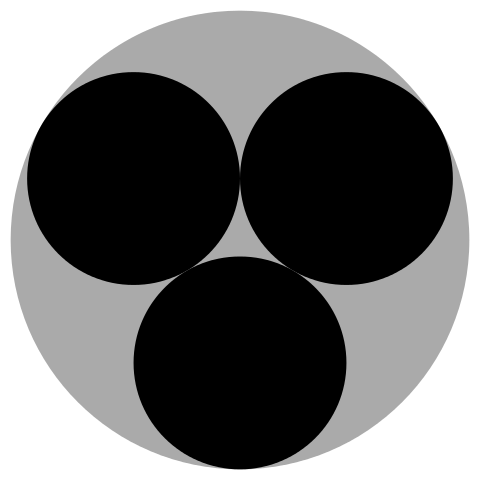
\includegraphics[width=5cm]{figures/bundle-3.png}
\end{center}
\caption{Circle packing where $n = 3$}
\label{bundles:bundle-3}
\end{figure}

\begin{figure}
\begin{center}
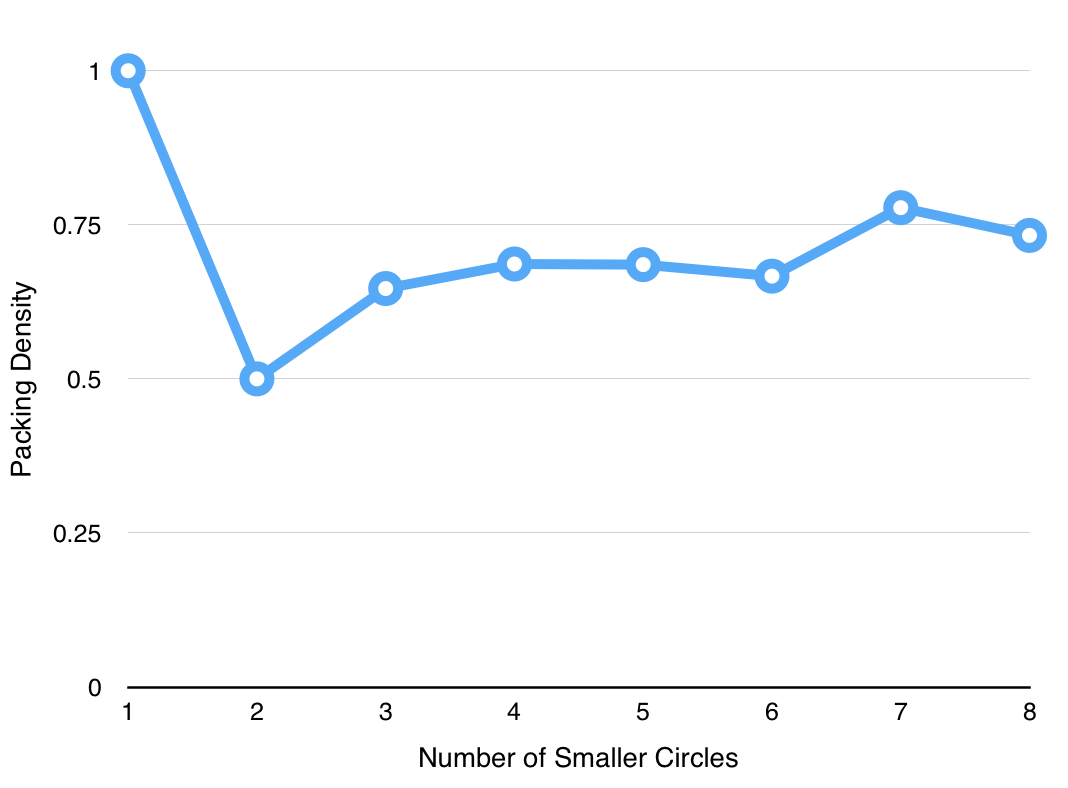
\includegraphics[width=10cm]{figures/density.png}
\end{center}
\caption{Packing density vs. number of smaller circles}
\label{bundles:density}
\end{figure}

The overall bundle shape is circular, and each individual spaghetti is also
circular.
To optimise the strength of the bundle (increase its maximum load) relative to
its mass, we must maximise the density of spaghetti within this larger circular
bundle shape.
A higher density of spaghetti will increase the tensile strength of the bundle,
increasing its maximum load relative to its mass.
Thus the problem reduces to solving for the maximum possible density of
smaller circles (the spaghetti) within a larger overall circle (the bundle).
In mathematics, this problem is called circle packing theory.

For example, the most optimal method of packing 3 small circles into a larger
circle is shown in Figure \ref{bundles:bundle-3}.
This configuration has a density of 0.6466.
This means that 64.66\% of the surface of the larger circle is covered by the
smaller circles.

Figure \ref{bundles:density} shows a graph of packing density vs. number of
smaller circles ($n$).
This graph appears very similar to that in Figure \ref{bundles:graph}, of load
to mass ratio of spaghetti bundles vs. bundle size, in that there is a general
decrease from $n = 1$ until $n = 7$, where it increases again before decreasing.

The configuration where $n = 7$ is the most dense (after $n = 1$) since it
consists of 6 circles forming a hexagon around a central circle.
This has a much higher density than any previous configuration.
This configuration next occurs at $n = 19$, where the next layer of the hexagon
is added.


\subsubsection{Conclusions}

From packing theory, we can draw the conclusion that a bundle size of 1 will
have the highest load to mass ratio, then a bundle size of 7, and then one of
size 3.
Using a bundle of size 19 is impractical due to its immense width.

Thus in our design, any important segments of spaghetti will be made from
bundles of size 7 (such as the base and two main arches), any important
connecting segments will be bundles of size 3, and smaller triangles will be
formed using single strands of spaghetti.




\section{Testing Configurations}

The next stage in pre-testing was to determine what class of bridge we would use
for our design.
The two classes of designs discovered during research that were feasible to
build from spaghetti were truss and arch bridges.

This test consisted of constructing a small scale truss and arch bridge and
subjecting each to an increasing load force, to determine which had the highest
load to mass ratio.


\subsection{Design}

Each bridge was constructed according to the set of specifications the final,
full scale bridge is subject to. The following changes were made to accomodate
for the smaller size of these testing bridges:

\begin{itemize}
\item The bridge is to span a gap of 10 cm.
\item The base is to be 20 cm in length.
\item The bridge is to be constructed using San Remo tubular spaghett.
\item The joints are to be formed using a juducious volume of hot glue.
\item The bridge is to be constructed from single strands of spaghetti (no
	bundles).
\end{itemize}

\begin{figure}
\begin{center}
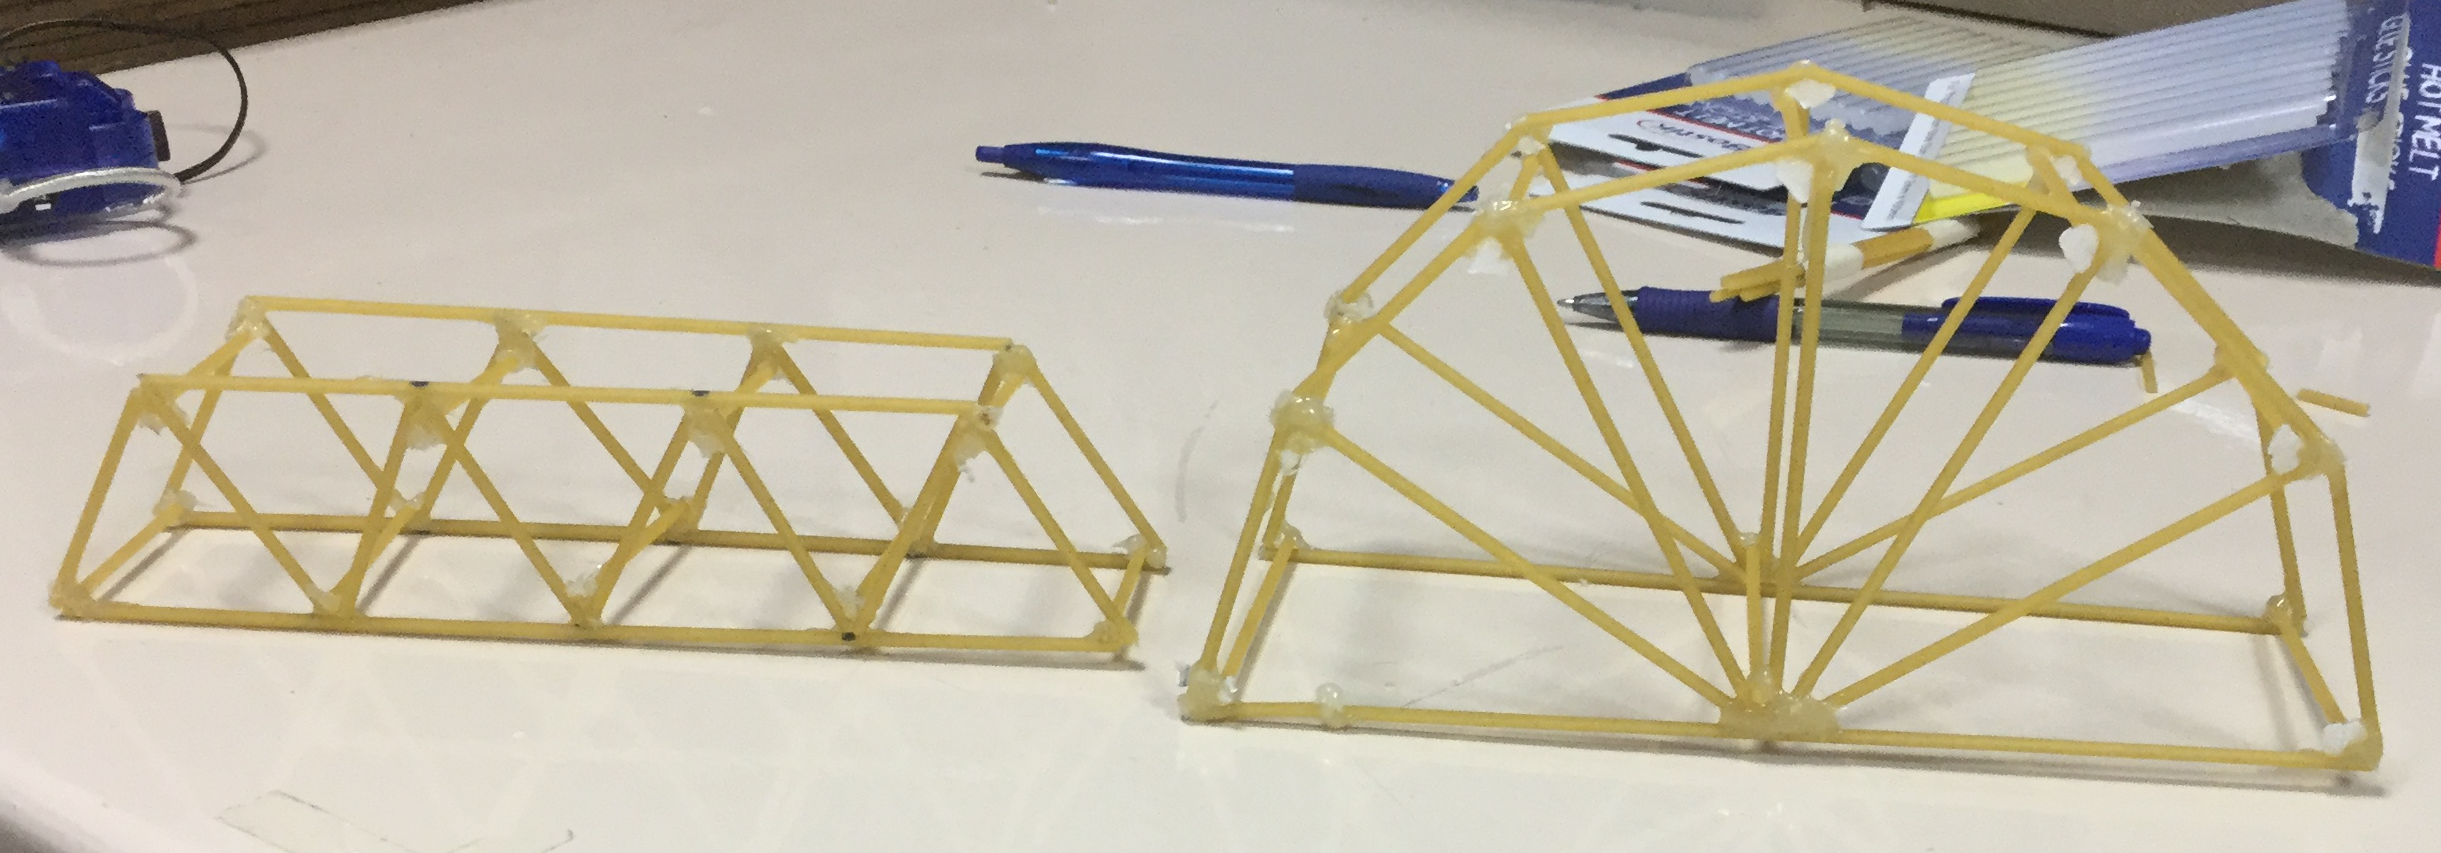
\includegraphics[width=\textwidth]{figures/config-photo.png}
\end{center}
\caption{A photograph of the arch and truss bridges}
\label{config:photo}
\end{figure}

A photograph of the small scale arch and truss bridge constructed can be seen
in Figure
\ref{config:photo}.


\subsection{Equipment}

The equipment required to conduct the testing of each bridge is as follows:

\begin{itemize}
\item GLX force metre and associated power pack
\item 2 tables of the same height
\item 2 heat proof mats
\item String
\item Electronic scales
\end{itemize}


\subsection{Procedure}

To test each bridge, the following procedure was conducted:

\begin{enumerate}
\item Place two tables together, separated by a gap of 10 cm.
\item Place a heat proof mat at the edge of each table (for the same reason as
	earlier).
\item Set up and calibrate the GLX force metre.
\item \label{config:start} Select one of the small scale bridges to test.
\item Record the mass of the bridge.
\item Place it across the gap, ensuring it is centred and overlaps each table
	by 5 cm.
\item Tie a loop of string around the width of the bridge.
\item Hook the GLX force meter around the loop of string.
\item Gradually pull vertically down until the bridge breaks.
\item \label{config:end} Record the maximum force at which the bridge broke.
\item Repeat steps \ref{config:start} to \ref{config:end} with the other small
	scale bridge.
\end{enumerate}


\subsection{Results}

\begin{center}
\makebox[\textwidth][c]{
\begin{tabular}{|C{0.2\textwidth}|C{0.2\textwidth}|C{0.2\textwidth}|C{0.2\textwidth}|C{0.2\textwidth}|}
\hline
Bridge Type & Mass ($\times 10^{-3}\mbox{ kg}$) & Force (N) & Effective Load
(kg) & Load to Mass Ratio \\
\hline
Truss & 14.4 & 20.2 & 2.061 & 143 \\
Arc   & 18.7 & 29.8 & 3.040 & 163 \\
\hline
\end{tabular}
}
\end{center}


\subsubsection{Sample Calculation}

A sample calculation for the load to mass ratio of the arc bridge is shown
below.

Effective load:

$$
\begin{aligned}
F & = ma \\
20.2 & = m \times 9.8 \\
m & = 2.061\mbox{ kg} \\
\end{aligned}
$$

Load to mass ratio:

$$
\begin{aligned}
& = \frac{2.061}{18.7 \times 10^{-3}} \\
& = 163 \\
\end{aligned}
$$


\subsection{Evaluation}

\begin{figure}
\begin{center}
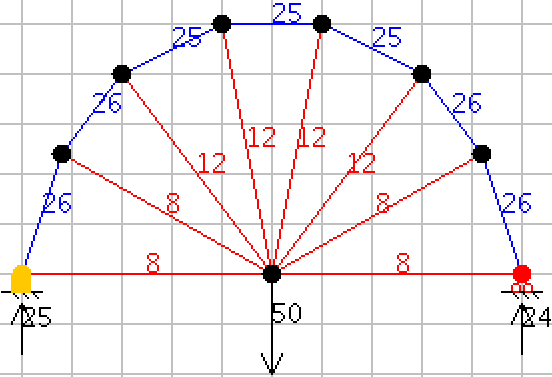
\includegraphics[width=5cm]{figures/arch-2.png}
\end{center}
\caption{The forces in an arch bridge}
\label{config:arch}
\end{figure}

\begin{figure}
\begin{center}
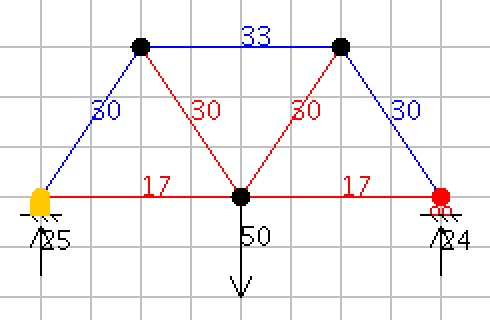
\includegraphics[width=5cm]{figures/truss-1.png}
\end{center}
\caption{The forces in a truss bridge}
\label{config:truss}
\end{figure}

The above data indicated that an arc bridge would be the most effective style of
bridge design, as it had a higher load to mass ratio than the truss bridge.

This is due to an arch bridge's design.
When subject to a high load force concentrated at the centre of its base, this
causes the spokes attached to the base and the arch to experience a tension
force.
The spokes closer to the centre of the arch will experience a larger tension
force than those attached near the edges of the arch, since these central spokes
have a larger component of their length in the direction opposite to that of the
load force applied (ie. the vertical direction).
These tension forces in the spokes cause compression forces in the segments of
the arch, which are distributed evenly amongst the segments.
This is demonstrated in Figure \ref{config:arch}.

In a truss design, the concentrated load force at the centre of its base causes
tension in the surrounding 4 spokes.
This creates a compression force in the upper segment of this inner triangle,
and in the outer segment of the two outer triangles.
This is demonstrated in Figure \ref{config:truss}.

Because of this, an arch's design is more effective than a truss in reducing
the overall tension and compression forces experienced by each segment in the
structure.
Since the bridge design will break once the tension or compression force in a
segment of spaghetti exceeds that piece of spaghetti's maximum tensile or
compressive strength, a reduction in the overall tension and compressive forces
for any given load will allow an arch bridge to sustain a larger load force
than a truss bridge of the same mass.


\subsection{Average Tension and Compression Force Per Unit Mass}

We can quantify this reduction in overall tension and compression forces in an
arch bridge compared to a truss using a computer simulation to calculate the
forces present in each type of bridge.
We will use the arch and truss bridge shown in Figures \ref{config:arch} and
\ref{config:truss} for this.

Firstly, we tabulate all tension and compression forces for each bridge type.
If we assume the linear mass density of the spaghetti to be constant (a
reasonable assumption), then by dividing each of these forces by the total
length of all members in the design, we can find an equivalent set of tension
and compression forces for each type.

We can then calculate the average, median, and standard deviation of these data
sets to show that an arch bridge is more effective in reducing the overall
tension and compression forces.
The standard deviation of these data sets acts as an indication as to how evenly
each design spreads its tension and compression forces amongst its segments of
spaghetti.
A lower standard deviation indicates that there is less variance in tension or
compression forces, implying that the design more evenly distributes the applied
load force.

% The bridge will fail if any one single length of spaghetti exceeds its maximum
% tension or compression force.
% If we only considered the average of these tension and compression forces,
% rather than the median and standard deviation, this would potentially hide any
% pieces of spaghetti experiencing a tension or compression high above the
% average (which could cause the bridge to fail).
% The standard deviation reflects the average variance in the data, thereby
% exposing any of these potential outliers.


\subsubsection{Truss Bridge}

The total length of all segments in the truss bridge is the sum of the 3
horizontal members, plus the length of the 4 diagonal sides of the triangles:

$$
\begin{aligned}
& = 3 \times 4 + 4 \times \sqrt{2^2 + 3^2} \\
& = 12 + 4\sqrt{13} \\
& = 26.42\mbox{ units} \\
\end{aligned}
$$

All tension forces are shown below:

\begin{center}
\begin{tabular}{|c|c|}
\hline
Tension Force (N) & Force Per Unit Mass ($\mbox{N kg}^{-1}$) \\
\hline
17 & 0.6456 \\
30 & 1.136 \\
30 & 1.136 \\
17 & 0.6456 \\
\hline
\end{tabular}
\end{center}

The average of this data set is $0.8908\mbox{ N kg}^{-1}$, the median
$1.136\mbox{ N kg}^{-1}$, and standard deviation 0.2831.

All compression forces are shown below:

\begin{center}
\begin{tabular}{|c|c|}
\hline
Compression Force (N) & Force Per Unit Mass ($\mbox{N kg}^{-1}$) \\
\hline
30 & 1.136 \\
33 & 1.249 \\
30 & 1.136 \\
\hline
\end{tabular}
\end{center}

The average of this data set is $0.9176\mbox{ N kg}^{-1}$, the median
$1.136\mbox{ N kg}^{-1}$, and standard deviation 0.06524.


\subsubsection{Arc Bridge}

The total length of all segments in the arch bridge (which has 7 segments) is
the length of the 8 radii, plus the length of the 7 segments.

The length of 1 segment can be calculated using the cosine rule, as the angle
between consecutive radii is $\frac{180}{7}$:

$$
\begin{aligned}
& = \sqrt{2 \times 5^2 - 2 \times 5^2 \times \cos{\frac{180}{7}}} \\
& = 2.225\mbox{ units} \\
\end{aligned}
$$

Thus the total length of all members in the arch bridge is:

$$
\begin{aligned}
& = 8 \times 5 + 7 \times 2.225 \\
& = 55.58\mbox{ units} \\
\end{aligned}
$$

All tension forces are shown below:

\begin{center}
\begin{tabular}{|c|c|}
\hline
Tension Force (N) & Force Per Unit Mass ($\mbox{N kg}^{-1}$) \\
\hline
8 & 0.1439 \\
8 & 0.1439 \\
12 & 0.2159 \\
12 & 0.2159 \\
12 & 0.2159 \\
12 & 0.2159 \\
8 & 0.1439 \\
8 & 0.1439 \\
\hline
\end{tabular}
\end{center}

The average and median of this data set is $0.1799\mbox{ N kg}^{-1}$, the
standard deviation 0.03849.

All compression forces are shown below:

\begin{center}
\begin{tabular}{|c|c|}
\hline
Compression Force (N) & Force Per Unit Mass ($\mbox{N kg}^{-1}$) \\
\hline
26 & 0.4678 \\
26 & 0.4678 \\
25 & 0.4498 \\
25 & 0.4498 \\
25 & 0.4498 \\
26 & 0.4678 \\
26 & 0.4678 \\
\hline
\end{tabular}
\end{center}

The average of this data set is $0.4601\mbox{ N kg}^{-1}$, the median
$0.4678\mbox{ N kg}^{-1}$, and standard deviation 0.009621.


\subsubsection{Comparison}

From this quantitive data above, it is fairly apparent that an arch design
reduces the average and median compression and tension forces present in the
structure for any given load, concentrated at the centre of the base. The
average for tension forces was $0.8908\mbox{ N kg}^{-1}$ and
$0.1799\mbox{ N kg}^{-1}$ for a truss and arch bridge respectively, and for
compression forces $0.9176\mbox{ N kg}^{-1}$ and $0.4601\mbox{ N kg}^{-1}$
respectively.

In addition, by considering the standard deviations of these data sets, we are
able to show that the variation in tension and compression forces in an arch
design is much less than that of a truss (for tension forces, the standard
deviations were 0.03849 and 0.2831 respectively; for compression, 0.06524 and
0.009621 respectively).
This suggests that an arch design is more effective at evenly distributing
tension and compression forces amongst its members.

The conclusion we can draw from this data, along with the previous test of
physical structures, is that an arc design will have a higher load to mass ratio
than a truss.




\section{Testing Arch Segments}

In accordance with the previous testing of configurations, it was decided that
an arch bridge would be most optimal.
In order to construct such a bridge, we would have to create two semi-circular
lengths of spaghetti to form two parallel arches. Spokes would then be attached
between each arch and the center of the base.

It was decided that these arches would be constructed by approximating their
shape using a number of small, straight segments of spaghetti glued together,
rather than attempting to create a long piece of spaghetti and bend it into a
semi-circular shape.
This is because, in order to bend a piece of spaghett, we would have had to
soften it by partially hydrating it, then hardening it again.
This would weaken the tensile and compressive strength of the spaghetti by
making it more brittle, a very undesirable outcome.

We used a computer simulation to determine the tension or compression force
present in each segment of the arch, and in each spoke connected to the base,
in order to find the optimal number of segments to approximate the
semi-circular arch with.

The simulation can be found at the following link:

\begin{center}
\url{http://pages.jh.edu/~virtlab/bridge/bridge.htm}
\end{center}


\subsection{Procedure}

\begin{enumerate}
\item \label{segments:start} Construct a bridge with 2 segments forming the
	arch (a triangle) in the simulator.
\item Ensure the radius of the arch (ie. the length of each spoke) is 10 units,
	and the length of the base is 20 units.
\item Place a load of 50 N onto the central node along the base (see diagrams
	below).
\item Calculate the forces present in each segment and spoke of the bridge
	using the interface provided by the simulator.
\item Average the compression force in each arch segment, and record this
	number.
\item \label{segments:end} Average the tension force in each spoke, and record
	this number.
\item Repeat steps \ref{segments:start} to \ref{segments:end}, increasing the
	number of segments in the arch by 1, until a maximum of 16 arch segments is
	reached.
\end{enumerate}


\subsection{Results}

\begin{center}
\begin{tabular}{|C{0.25\textwidth}|C{0.25\textwidth}|C{0.25\textwidth}|}
\hline
Number of Arch Segments & Average Spoke Tension (N) & Average Segment
Compression (N) \\
\hline
2  & 34.0 & 35.0 \\
3  & 26.3 & 32.3 \\
4  & 19.0 & 30.0 \\
5  & 15.7 & 29.6 \\
6  & 12.2 & 28.3 \\
7  & 10.9 & 27.0 \\
8  & 9.7  & 25.5 \\
9  & 7.9  & 25.3 \\
10 & 6.1  & 25.4 \\
11 & 5.3  & 25.3 \\
12 & 5.0  & 25.3 \\
13 & 4.8  & 25.3 \\
14 & 4.7  & 25.3 \\
15 & 4.7  & 25.2 \\
16 & 4.6  & 25.2 \\
\hline
\end{tabular}
\end{center}

\begin{figure}
\begin{center}
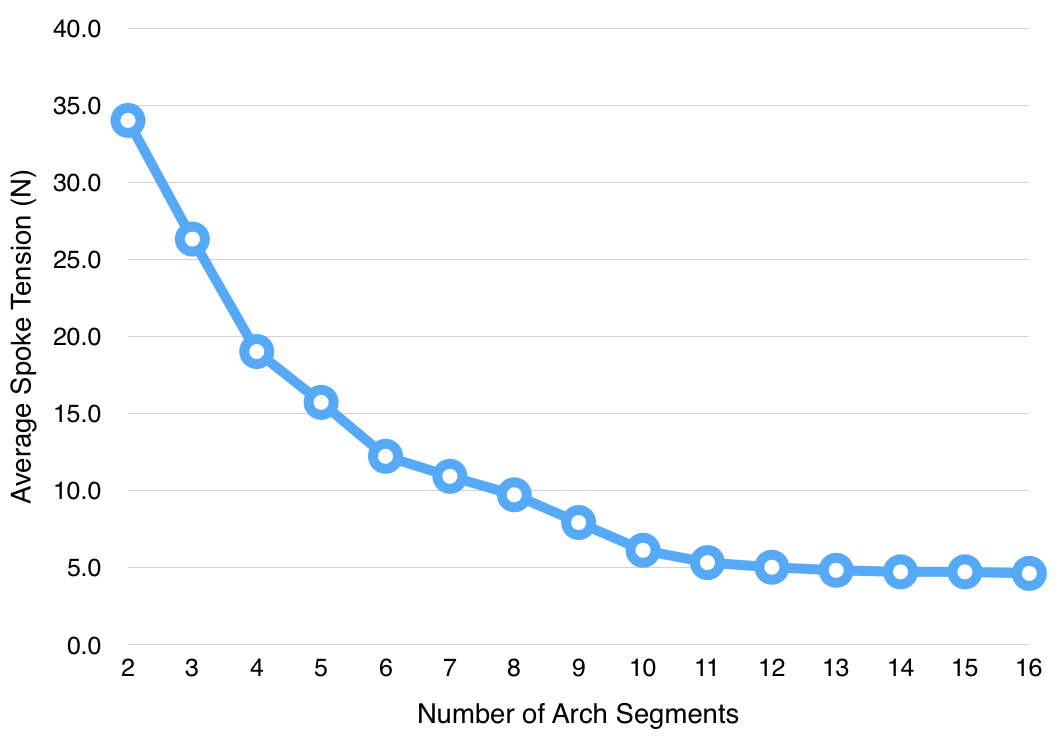
\includegraphics[width=10cm]{figures/spokes.png}
\end{center}
\caption{Average spoke tension vs. number of arch segments}
\end{figure}


\begin{figure}
\begin{center}
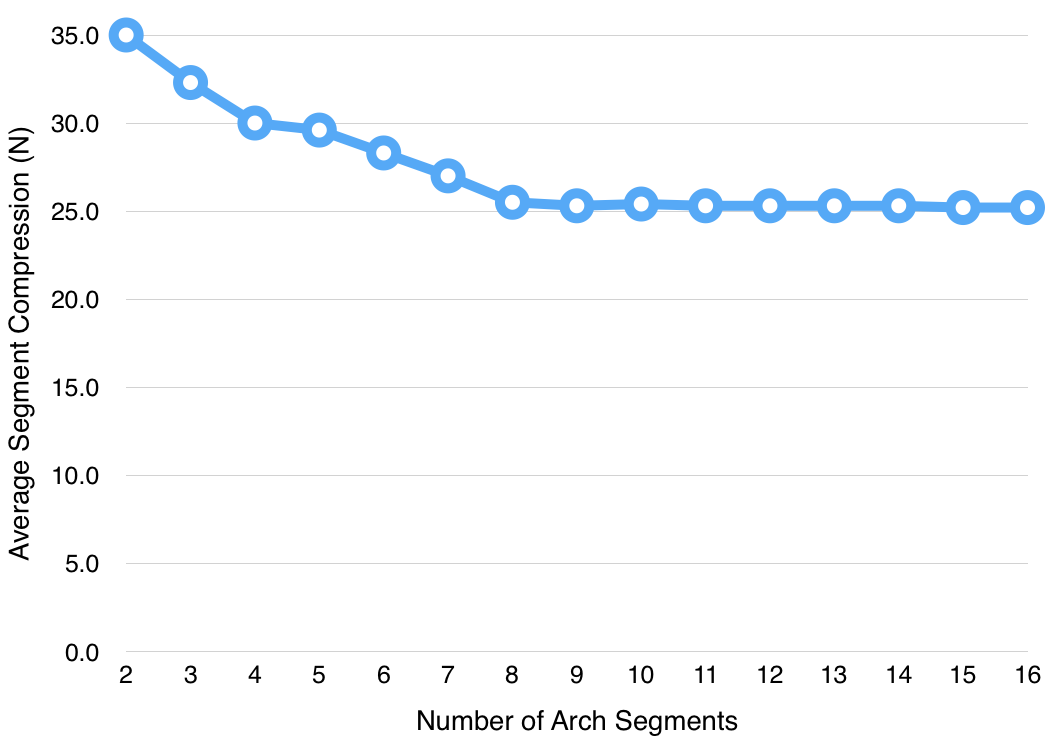
\includegraphics[width=10cm]{figures/segments.png}
\end{center}
\caption{Average segment compression vs. number of arch segments}
\end{figure}


\subsection{Evaluation}

\subsubsection{Decreasing Force}

The clearest trend in the results is that as the number of arch segments
increases, the average tension force in each spoke, and the average compression
force in each arch segment decreases.

This is likely due to the fact that as the number of arch segments increases,
the shape of the bridge becomes a better approximation of a semi-circle.
A semi-circular bridge can carry high load forces as it distributes the tension
forces in the spokes outwards as compression forces in the segments of the arch,
spreading the load force to the table at either edge.

This trend indicates that, in order to achieve an optimal load to mass ratio for
our bridge, we should be approximating a semi-circle with a relatively large
number of segments.


\subsubsection{Parity of the Number of Segments}

\begin{figure}
\begin{center}
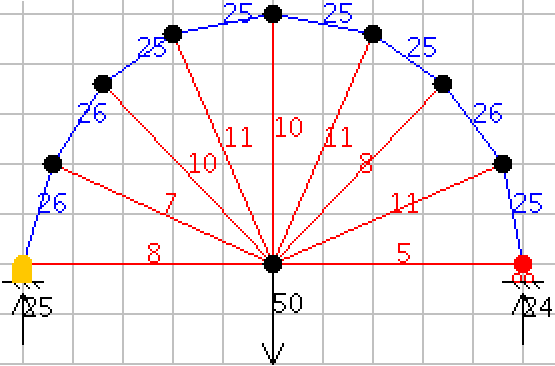
\includegraphics[width=5cm]{figures/arch-1.png}
\end{center}
\caption{An arch with 8 segments}
\label{arch:8-segments}
\end{figure}

\begin{figure}
\begin{center}
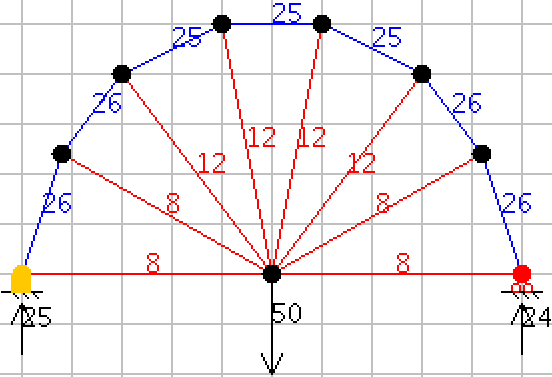
\includegraphics[width=5cm]{figures/arch-2.png}
\end{center}
\caption{An arch with 7 segments}
\label{arch:7-segments}
\end{figure}

The parity of the number of arch segments (whether we have an even or odd number
of segments) is also significant.)

In an arch with an even number of segments, such as in Figure
\ref{arch:8-segments}, there exists a single spoke extending from the top of
the arch, joining the centre of the base at a $90^\circ$ angle.

In an arch with an odd number of segments, there are two spokes extending from
the top of the arch, meeting the base at the same angle, such as in Figure
\ref{arch:7-segments}.
In such an arch, the tension forces in the spokes are more evenly distributed
amongst the central spokes than in an arch with an even number of segments.
This increases the strength of the design, increasing its potential load to mass
ratio.

Thus we will select a design with an odd number of arch segments.


\subsubsection{Decreasing Rate of Change of Force}

Another trend in the results is that as the number of arch segments increases,
the rate of change of force for both the spokes and segments decreases,
eventually levelling out at a value (4.6 N and 25.2 N for the spokes and
segments respectively).

This indicates that, past a certain number of arch segments, the marginal
decrease in tension and compression force from adding one more arch segment is
relatively insignificant when compared to the difficulty of constructing such an
arch. Thus there is an optimal number of arch segments to use such that we
achieve a relatively low tension and compression force, without making such a
bridge horrendously difficult to build.

For a bridge of 11 arch segments, the average segment compression
force has effectively levelled out, and the average spoke tension force is
relatively close to its minimum.
Such a bridge is also not overly time consuming to construct.

Thus we chose to build an arch of 11 arch segments, because:

\begin{itemize}
\item 11 segments is an odd number, thus elmininating a single spoke extending
	from the top of the arch to the base.
\item An arch of 11 segments is not too difficult or time consuming to
	construct.
\item It achieves relatively low tension and compression forces in the spokes
	and arch segments, as demonstrated by the computer simulation.
\end{itemize}




\section{Construction}

\subsection{Final Design}

The final design of the bridge was to be a semi-circular arch bridge of 11
segments.

The height of the arch was decided by the maximum length of the available
spaghetti to be used as spokes connecting the arches to the base.
This, on average, was just over 25 cm.
Thus the base of the arch was to be 50 cm in length, leaving 5 cm of bridge
overlapping the table either side of the 40 cm gap.

The width of the arch was decided to be the minimum length possible, in order to
reduce the weight of the bridge.
The bridge must be capable of carrying a 5 cm wide car along it.
Thus the inner width of the base was to be 5 cm.
The external width of the base would be larger (by 1.6 cm) due to the width of
the two arches attached to either side of the base.


\subsection{Arch Internal Angle}

\begin{figure}
\begin{center}
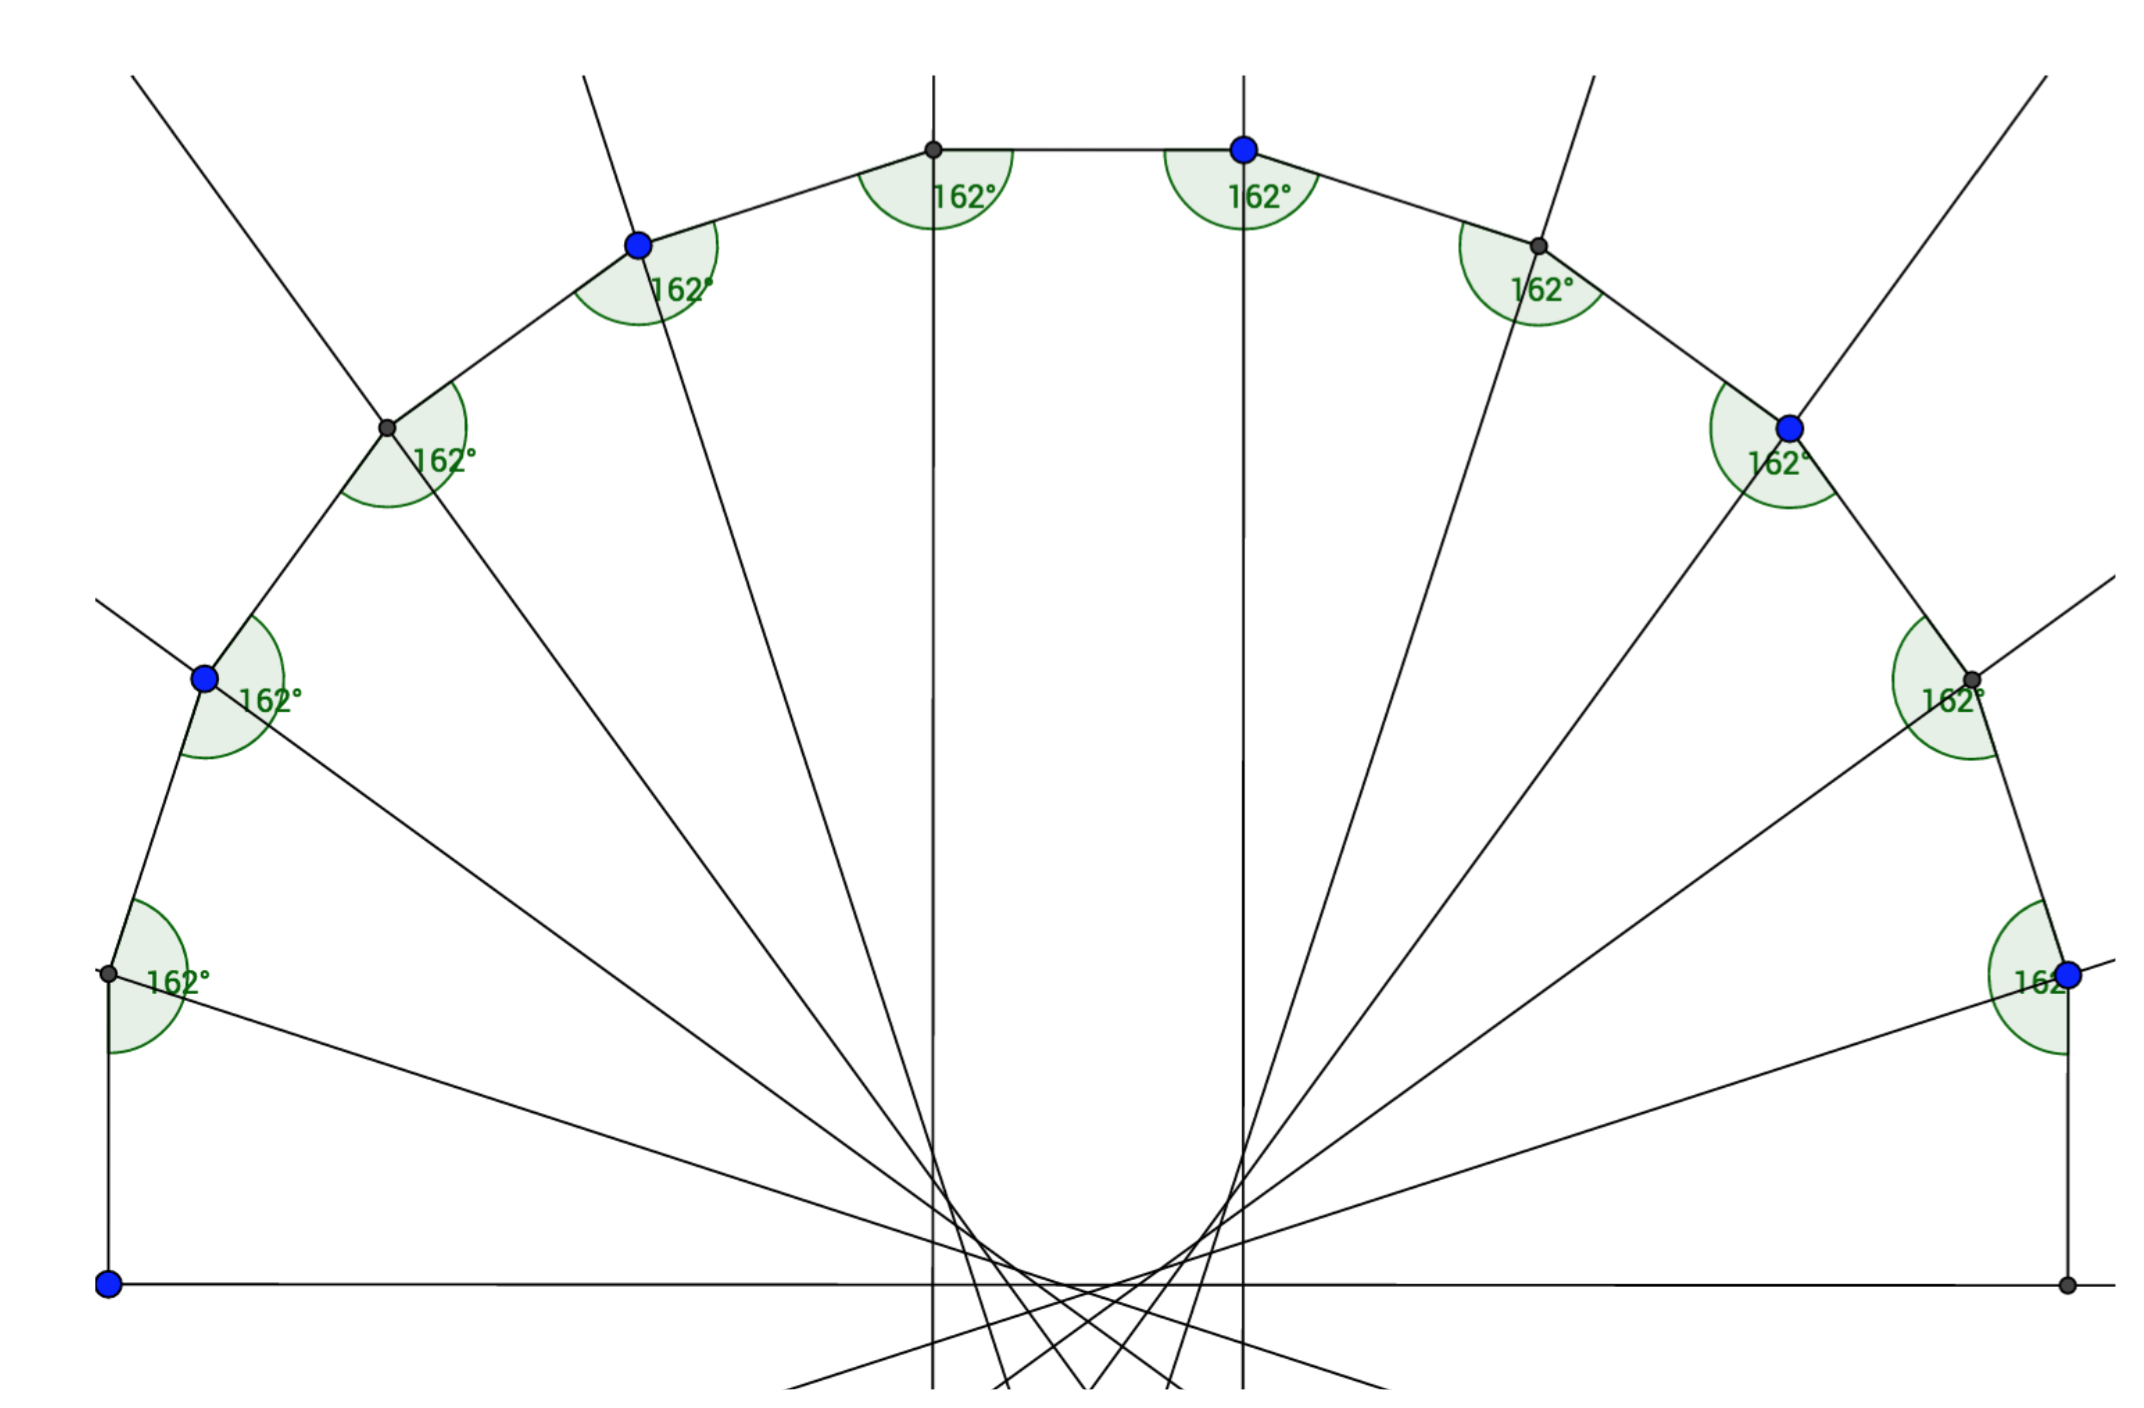
\includegraphics[width=10cm]{figures/schematic.png}
\end{center}
\caption{Arch schematic}
\label{construction:schematic}
\end{figure}

To create an effective semicircular bridge shape, the two initial segments of
the arch were designed to be perpendicular to the base.
In order to achieve this, we required 11 segments of an icosagon (a 20 sided
polygon) - 1 more segment than half of the polygon.
This can be seen in the schematic shown in Figure \ref{construction:schematic}.

The internal angle of an icosagon is given by:

$$
\begin{aligned}
& = \frac{180(n - 2)}{n} \\
& = \frac{180 \times 18}{20} \\
& = 162^\circ \\
\end{aligned}
$$

Thus each interior angle in the arch was to be $162^\circ$, as shown in the
schematic.


\subsection{Bundle Sizes}

As mentioned in the previous testing section, the most important parts of the
bridge were made from bundles of 7 spaghetti.
These consisted of the outer rectangle of the base of the bridge, the joining
lengths between the two sides of the base, and the two arches.

More minor components were made out of bundles of 3 spaghetti, and
included diagonal joins along the base, and horizontal joins between the two
arches.

Components formed from single strands of spaghetti include the diagonals between
horizontal joins between the two archs, and the spokes connecting the arches to
the base.


\subsection{Base Construction}

\begin{figure}
\begin{center}
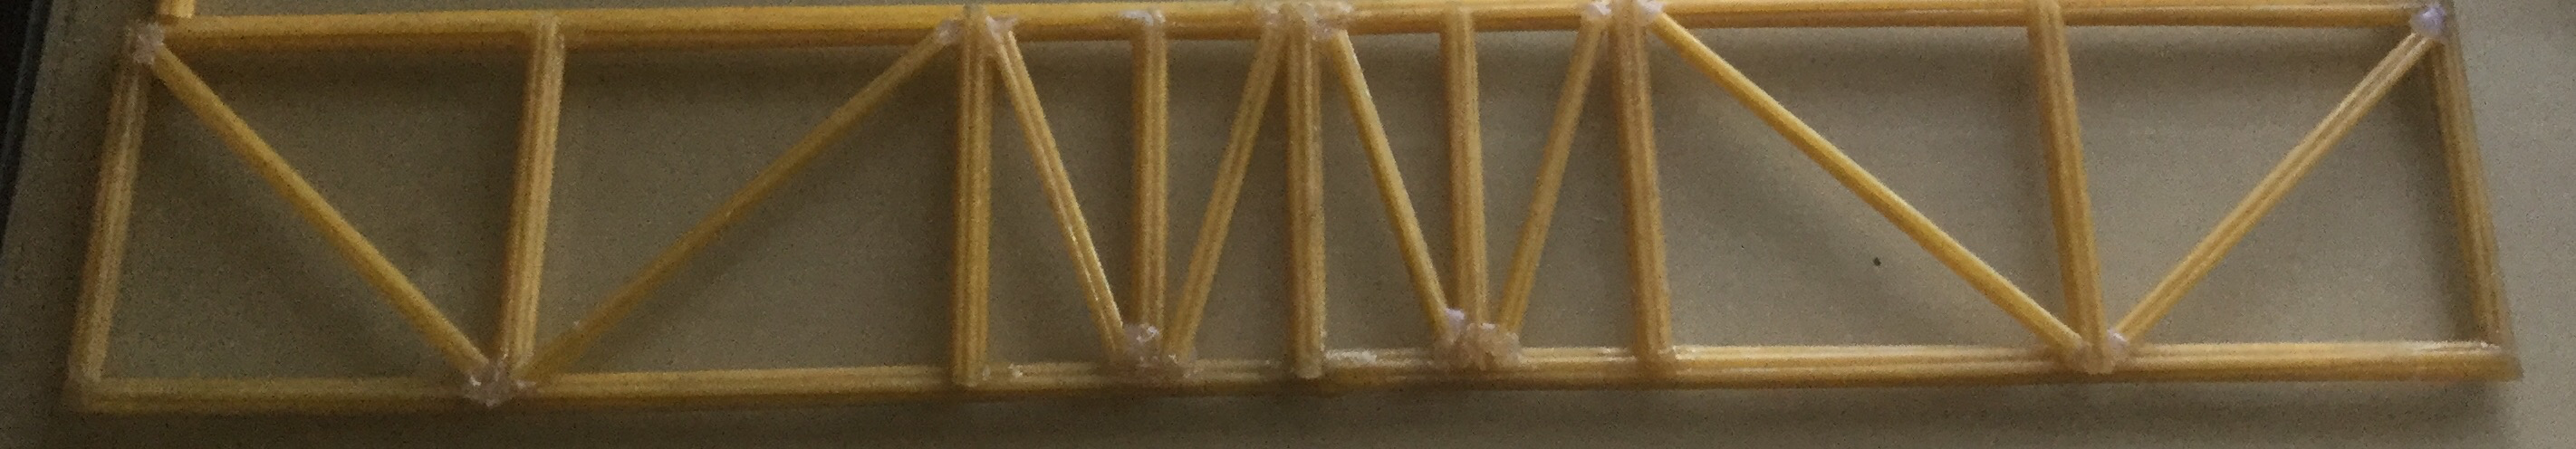
\includegraphics[width=\textwidth]{figures/base.png}
\end{center}
\caption{Photograph of base}
\label{construction:base}
\end{figure}

\begin{figure}
\begin{center}
\includegraphics[width=\textwidth]{figures/constructed-bundles.png}
\end{center}
\caption{The angled ends of the spaghetti bundles}
\label{construction:bundles}
\end{figure}

\begin{figure}
\begin{center}
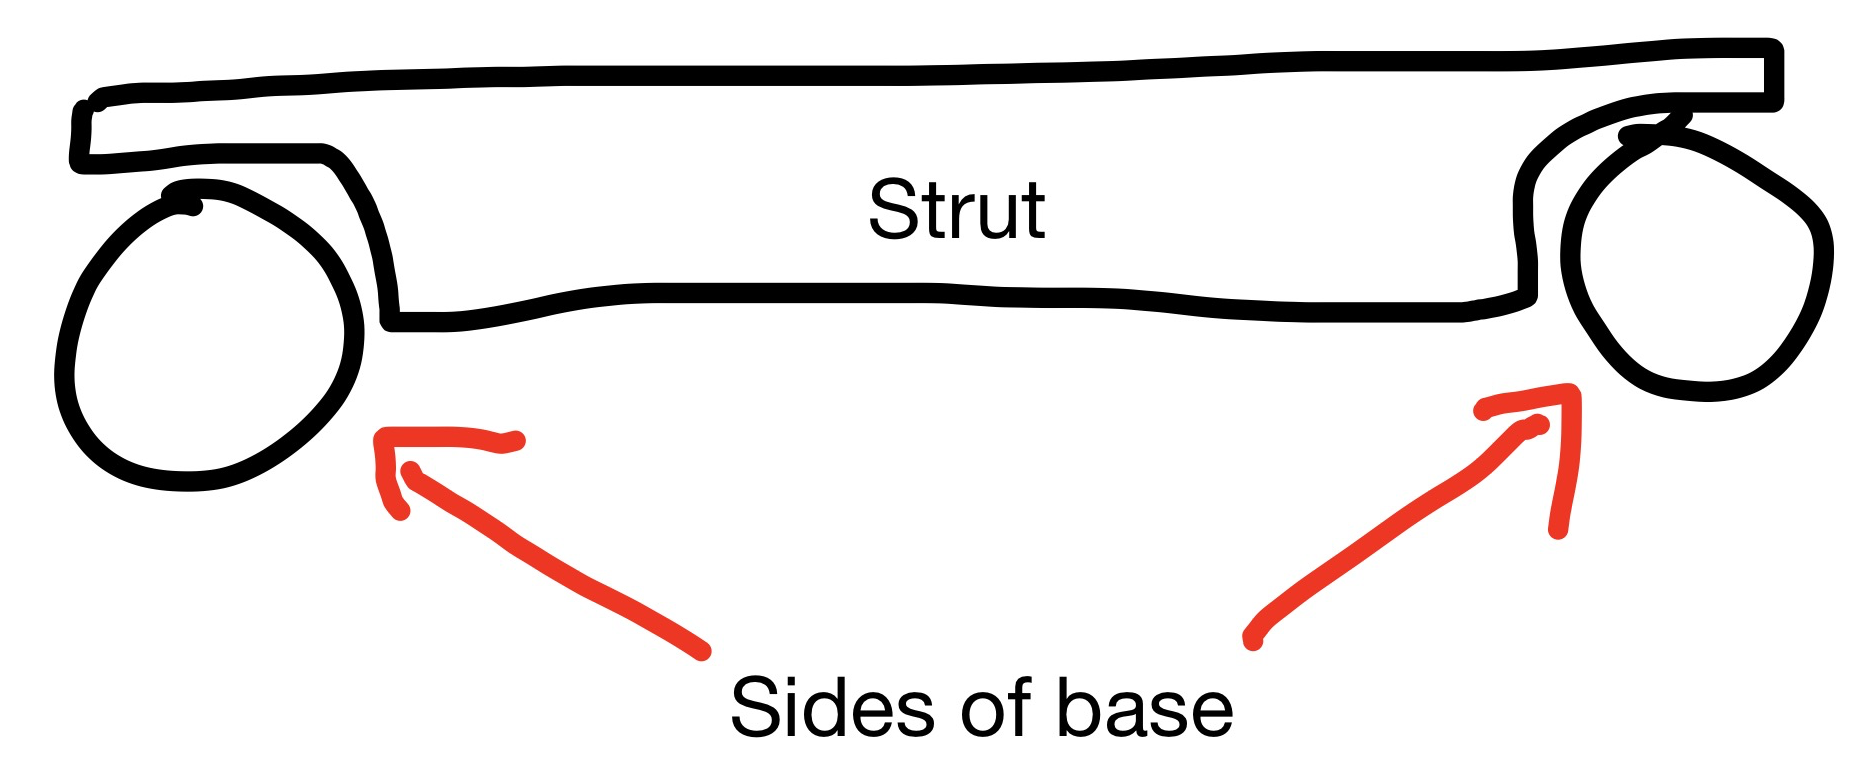
\includegraphics[width=\textwidth]{figures/struts.png}
\end{center}
\caption{The horizontal struts that sit across the base}
\label{construction:struts}
\end{figure}

The first component of the bridge we constructed was the base.
A photograph of the completed base is shown in Figure \ref{construction:base}.

Firstly, the outer rectangle of the base was constructed from bundles of
spaghetti of size 7.
These bundles were created by applying Araldite epoxy to the ends of a group of
7 spaghetti, then binding it with masking tape and letting the glue set.

The two 50 cm side lengths were formed by joining two 25 cm bundles.
Each end of each bundle was sanded using an electric belt sanding machine to
achieve an angle of $45^\circ$, before applying epoxy to join the two pieces.
This angled sanding flattened the ends of the bundles, allowing both pieces to
fit together easily. It also increased the available surface area for contact
between the two pieces, increasing the area over which the glue could adhere to.
This increased the strength of the joint.
A photograph of these angled ends of the spgaghetti bundles is shown in Figure
\ref{construction:bundles}.

The two side lengths were joined by 5 cm lengths of spaghetti bundles at either
end. The edges of these were also sanded to $45^\circ$ for the aforementioned
reasons.

Finally, shorter bundles of 7 spaghetti were placed horizontally across the base
to ensure its structural integrity and rigidity.
Since the load force would be applied onto these struts through the strapping
tape that was to hang over them, we required them to be extremely strong.
The ends of these segments were shaped using a circular metal file such that
they would sit on top of the side lengths of the base, which can be seen in
Figure \ref{construction:struts}.
They were then joined to the base using epoxy.
We also increased the frequency of these struts at the centre of the base,
where the load would be suspended from, to ensure the base would not fail.


\subsection{Arch Segments}

A diagram of an arch segment:

\vspace{4cm}

To construct the arch, 11 segments of spaghetti bundles were needed.
The length of these pieces of spaghetti, assuming the radius of the arch is 25
cm, can be calculated by the cosine rule:

$$
\begin{aligned}
& = \sqrt{2 \times 25^2 - 2 \times 25^2 \cos{\frac{180}{11}}} \\
& = 7.12\mbox{ cm} \\
\end{aligned}
$$

In order to have the arch curve around once the segments were fitted together,
we needed to sand one end of each segment to a particular angle, assuming the
other end was left at $90^\circ$.
This angle is calculated by:

$$
\begin{aligned}
& = 360 - 90 - 162 \\
& = 108^\circ \\
\end{aligned}
$$

This is shown in the above diagram.

These pieces were fashioned from bundles of spaghetti of size 7, and sanded to
the correct length and with the correct angles.
The arches were initially glued using hot glue, as we could easily adjust the
joins between segments in order to have the two arches line up exactly.
Once this was complete, the joints were coated in epoxy to increase their
rigidity (as mentioned earlier).


\subsection{Spokes}

\begin{figure}
\begin{center}
\includegraphics[width=\textwidth]{figures/final.png}
\end{center}
\caption{Photograph of constructed bridge}
\label{construction:final}
\end{figure}

After constructing the base and two arches, these were joined together using
epoxy.
Spaghetti bundles of size 3 were glued horizontally at each of the 10 joints
between arch segments to ensure the arches remained upright and in a rigid
position.
Again, hot glue was used initially to ensure the placement of each of these
segments was correct, before the joints were coated in epoxy and left to dry.
These bundles were cut to size using a pair of pliers as the bridge was built,
to ensure a perfect fit.

Diagonals constructed from single strands of spaghetti were then glued between
each of these horizontal segments, again using hot glue initially, before
coating in epoxy.
Again, pliers were used to cut these strands as the bridge was constructed.

Single strands of spaghetti were then connected between each of the 10 arch
segments and the base, initially using hot glue, before coating each joint in
epoxy.
These were also cut to size using the pliers as construction progressed.

All gluing at this stage was performed on top of baking paper, as it was found
that neither the hot glue nor the Araldite epoxy adhered to it.
This allowed us to leave the structure in one position for the glue to set,
without worrying about having to remove it from the table or a piece of paper.

A final photograph of the bridge can be seen in Figure \ref{construction:final}.




\section{Failure}

\subsection{Load to Mass}

Our final bridge had a mass of 251.06 g, and supported a load of 25 kg.
Thus the load to mass ratio was:

$$
\begin{aligned}
& = \frac{25}{251.06 \times 10^{-3}} \\
& = 99.6 \\
\end{aligned}
$$

This was an appreciable achievement for such a comparatively heavy bridge.


\subsection{Failure Points}

\begin{figure}
\begin{center}
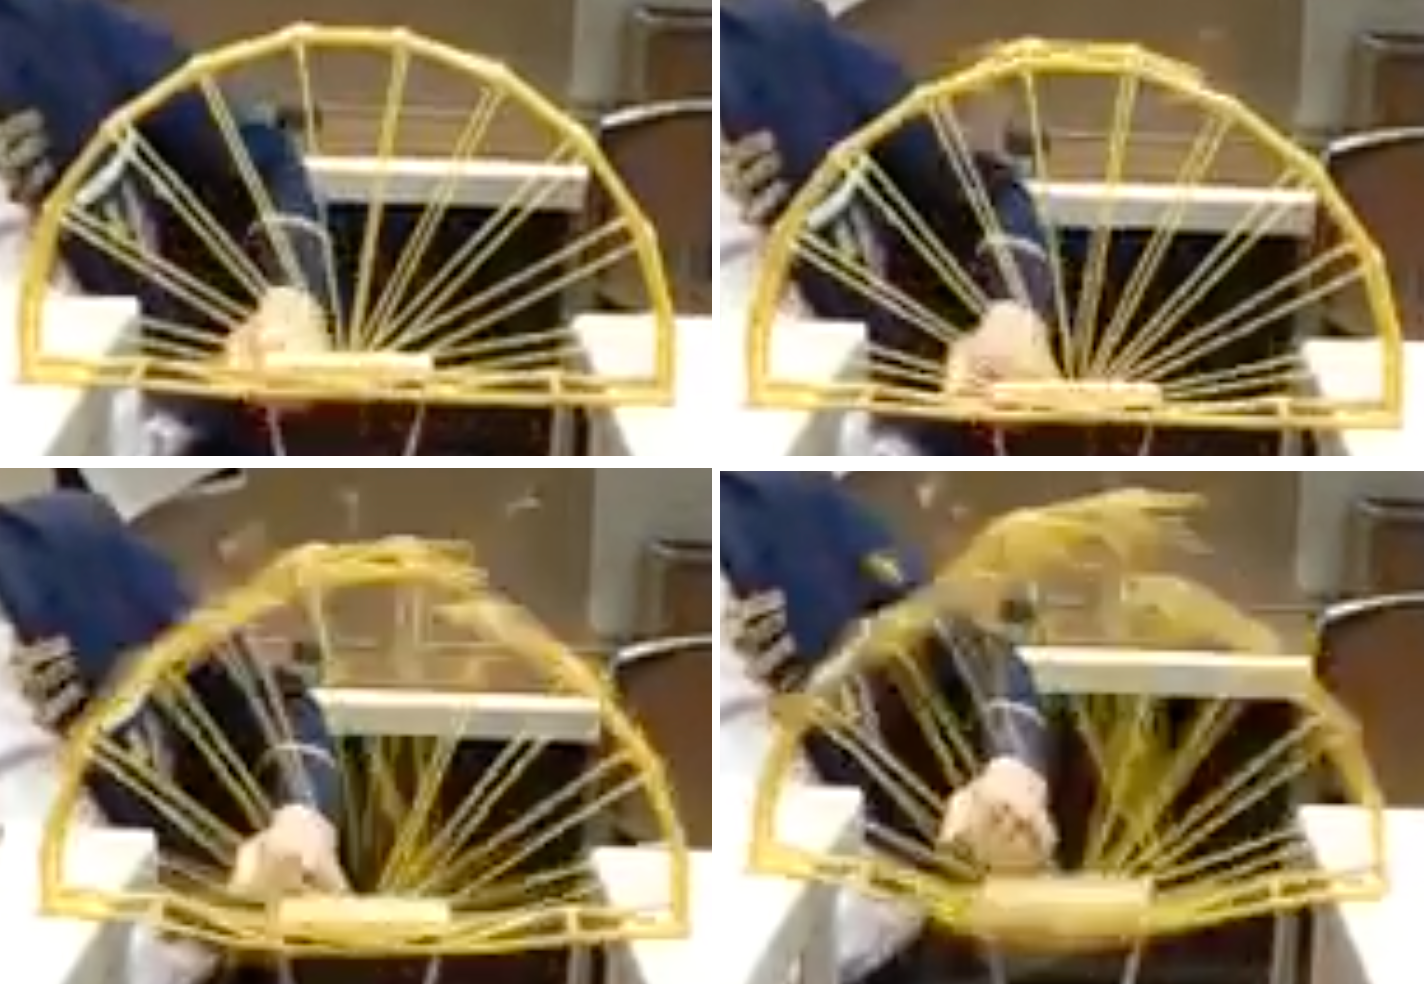
\includegraphics[width=10cm]{figures/frames.png}
\end{center}
\caption{Frame by frame analysis of bridge failure}
\label{failure:frames}
\end{figure}

A frame by frame analysis of the bridge as it broke is shown in Figure
\ref{failure:frames}.

As can be seen, the failure point occurred at one of the segments in the arch
furthest from the camera - specifically, the segment to the right of the
central one in the image.
This breakage would have resulted in the rear arch collapsing, applying large
torsion forces on the remaining spokes, and the closer arch.
This in turn caused the closer arch to fail, causing the bridge to collapse
inwards and for the base to break as the attached load fell to the ground.


\subsubsection{Arch Segment}

Earlier, when conducting research into bridge design, we noted that the
compressive strength of spaghetti is relatively weaker than its tensile
strength (spaghetti is better at withstanding tension forces than compressive
ones).
Since the segments of the arch are under compression, whereas the spokes and
base of the bridge were under tension, it is logical that the failure point of
our bridge would be in the arch.
This is confirmed by the fact that the bridge, once broken, begins to collapse
inwards starting at the top of the arch.


\subsubsection{Location of Segment}

The arch segment that failed was offset towards the right from the centre of
the bridge.
This implies that our construction of the bridge was slightly asymmetric,
subjecting the right side of the arch to slightly greater compressive forces
than the left, causing it to fail sooner.

In addition, it can be deduced from the images above that the failing arch
segment was one on the far side of the bridge, releative to the camera.
The top right image in Figure \ref{failure:frames} shows the closer arch
remaining intact, as the one behind it begins to break.
This implies that the farther arch was weaker in its construction than the
closer one, suggesting the two arches were not identical.

The segment that broke was also located near the top of the arch.
This breakage location was unexpected, considering that these top segments
undergo lesser compression forces than those nearer to the base.
This is because lower arch segments must sustain the compressive forces exerted
on them by a larger number of other segments above them.
This can be seen in Figure \ref{arch:8-segments}, where arch segments closer to
the base experienced slightly higher compression forces.
This unexpected breakage point suggests that the construction of the arches was
inaccurate in such a way that it increased the compression forces experienced by
segments of the arch near the top of the bridge.


\subsubsection{Base}

As the arch failed, the base, as seen in Figure \ref{failure:frames}, remained
intact, simply sagging at its centre, where the load force was applied.
This suggests that our base would have been able to continue to sustain higher
load forces had the arch not collapsed.


\subsubsection{Spokes}

Additionally, the spokes connecting the arches to the base also remained
relatively intact for a few moments after the arch began to fail.
This suggests that the spokes, similar to the base, were capable of withstanding
a higher load force before failure, had the arch not broken.




\section{Improvements}

\subsection{Design}

Several possible design changes would work to improve the overall compressive
strength of the arch segments in the bridge (this was the initial failure
point in our design).

The most significant one would be to increase the number of arch segments from
11 to (for example) 15 segments.
This would decrease the average compression force across the segments as the
arch becomes a better approximation of a semi-circle.
This would allow for the bridge to sustain a higher load.

In addition, an increased number of segments would also increase the number of
spokes between the arches and the base, decreasing the average tension in these
spokes, further improving the bridge's load carrying capabilities.

Finally, a larger number of arch segments would decrease the length of each.
Shorter pieces of spaghetti have a higher buckling strength, as noted in the
initial research section of this investigation.
This would increase the maximum compression force each segment could withstand
before breaking, increasing the maximum load force the bridge could sustain
before breaking, increasing its load to mass ratio.

A second possible improvement, although largely impractical, would be to
increase the number of spaghetti used in the bundles the arches were constructed
from.
The next highest bundle size with a high packing density is 19 spaghetti, as
discussed earlier.
This would increase the total compression force (independent of mass) each
segment of arch could withstand before breaking, without sacrificing the load to
mass ratio of the bridge.


\subsection{Gluing}

During the construction of our bridge, we coated several joints multiple times
with epoxy.
This lead to use of excessive volumes of glue in many cases, increasing the
overall mass of the bridge unnecessarily, and reducing the bridge's aesthetic
appeal.

An improvement on the bridge's design would be to reduce the amount of epoxy
used in coating each joint, to decrease its mass and improve its aesthetic
appearence.


\subsection{Bundles}

To construct the many bundles of 7 spaghetti in our bridge, we glued 25 cm
lengths of spaghetti together by placing glue at regular 8 cm intervals, letting
it set, and then sawing the bundles into multiple pieces using a bansaw
afterwards.
In some cases, the inaccurate placement of glue within the middle of these long
bundles meant that, once cut, some ends of several segments had very little
epoxy holding them together.
This would have reduced the strength of the segment, and the overall load to
mass ratio of the bridge.

An improvement would be to firstly measure and cut 7 individual strands of
spaghetti of the required length, and then to epoxy these together, to ensure a
sufficient amount of glue is used in forming each bundled segment.



\section{Conclusion}

Through the careful testing of various spaghetti and glue types, and bridge
structures and designs, we were able to construct a spaghetti bridge which,
which tested, had a load to mass ratio of 99.6.



\section{Bibliography}

A list of website links used for research and testing are listed below:

\begin{itemize}
\item \url{http://pghbridges.com/basics.htm}
\item \url{http://engineering.jhu.edu/ei/wp-content/uploads/sites/29/2014/01/Spaghetti-Bridge-Construction-Hints.pdf}
\item \url{http://www.warwickallen.com/bridges/ArchBridges.htm}
\item \url{http://science.howstuffworks.com/engineering/civil/bridge5.htm}
\item \url{https://en.wikipedia.org/wiki/Arch_bridge}
\item \url{http://www2.hesston.edu/Physics/ArchBridge/research.htm}
\item \url{https://en.wikipedia.org/wiki/Truss_bridge}
\item \url{http://ojhsbridges.weebly.com/truss-bridges.html}
\item \url{http://pages.jh.edu/~virtlab/bridge/bridge.htm}
\item \url{http://people.virginia.edu/~pjm8f/engr162/beam/stress_and_strain.htm}
\end{itemize}

\end{document}
